\documentclass{article}
\usepackage[T1]{fontenc}
\usepackage{lmodern}
\usepackage{graphicx}
\usepackage{amsmath,amssymb}
\usepackage[a4paper,margin=2cm]{geometry}
\usepackage[absolute,overlay]{textpos}
\setlength{\TPHorizModule}{1mm}
\setlength{\TPVertModule}{1mm}
\usepackage[indonesian]{babel}
\usepackage{hyperref}
\setlength{\emergencystretch}{2em}
% unit: Halaman 37

\begin{document}

% === Halaman 37 (llm) ===

\begin{itemize}
    \item \textbf{Wiretapping}
\end{itemize}

\vspace{60mm}

Baca di sini:
\begin{enumerate}
    \item \url{https://hackaday.com/2008/06/19/wiretapping-and-how-to-avoid-it/}
    \item \url{https://edition.cnn.com/videos/us/2017/03/07/what-is-wiretapping-jpm-orig.cnn}
\end{enumerate}

% deskripsi: Diagram ilustrasi cara kerja penyadapan telepon (simple line tap) yang menunjukkan koneksi antara power supply, alat wiretap, dan telepon.
% bbox normalisasi: [0.2180, 0.1840, 0.8570, 0.7340]
\begin{textblock*}{134.19mm}(45.78mm,54.65mm)
\noindent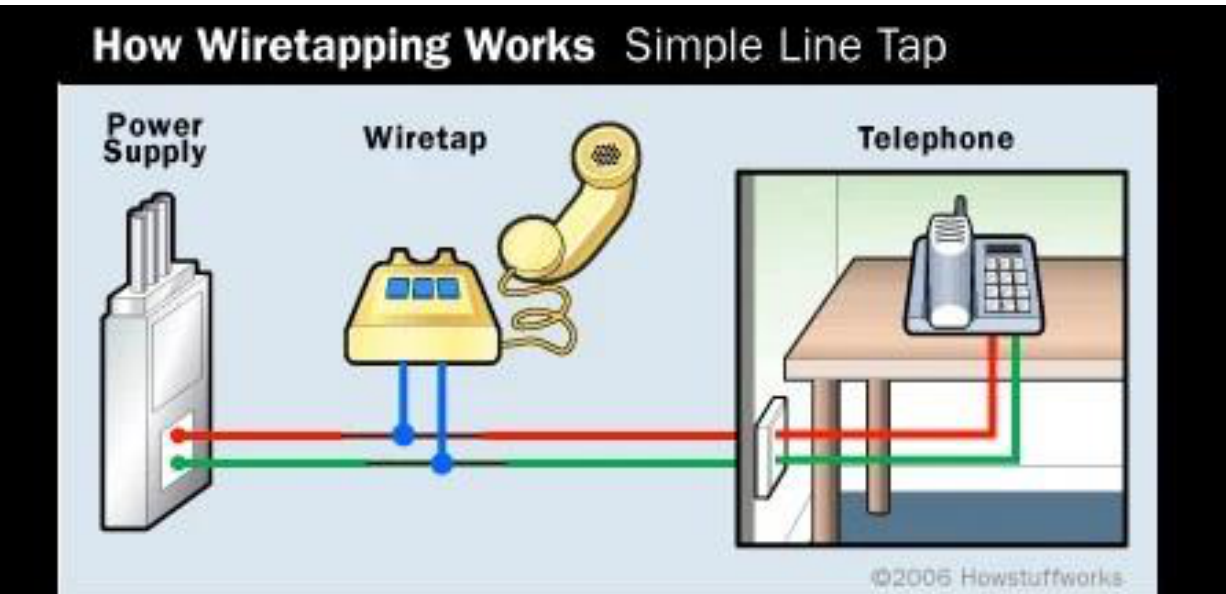
\includegraphics[width=134.19mm,height=163.35mm]{../../images/llm/page_037_img_01.png}%
\end{textblock*}

\end{document}
